% Avance 1 · Detección de celdas solares defectuosas en imágenes EL · PDI 2026-III
% Compilar desde esta carpeta:  latexmk -pdf presentacion.tex
% Mismo estilo que la presentación de la propuesta. Figuras: reports/figures (generadas por los scripts).
\documentclass[aspectratio=169,11pt]{beamer}

\usepackage[T1]{fontenc}
\usepackage[utf8]{inputenc}
\usepackage{lmodern}
\usepackage[spanish,es-noshorthands,es-nodecimaldot]{babel}
\usepackage{amsmath,amssymb}
\usepackage{booktabs}
\usepackage{array}
\usepackage{tikz}
\usetikzlibrary{positioning,arrows.meta}

\graphicspath{{../../reports/figures/}{../comun/}}

% ------------------------------------------------------------------ estilo (igual a la propuesta)
\definecolor{ud}{RGB}{128,57,61}
\definecolor{udsoft}{RGB}{242,230,231}
\definecolor{tinta}{RGB}{64,64,64}
\definecolor{gris}{RGB}{120,120,120}
\definecolor{caja}{RGB}{244,244,244}
\definecolor{okc}{RGB}{27,140,96}

\usefonttheme{serif}
\setbeamertemplate{navigation symbols}{}
\setbeamercolor{normal text}{fg=tinta}
\setbeamercolor{structure}{fg=ud}
\setbeamercolor{alerted text}{fg=ud}
\setbeamerfont{frametitle}{size=\Large,series=\bfseries}
\setbeamerfont{framesubtitle}{size=\small}

\setbeamertemplate{frametitle}{%
  \vskip0.25cm
  \begin{beamercolorbox}[wd=\paperwidth,leftskip=-0.15cm]{frametitle}%
    \begin{minipage}[c]{1.75cm}\centering
\includegraphics[height=1.15cm]{logo.png}\end{minipage}%
    \hspace{0.35cm}%
    \begin{minipage}[c]{0.78\paperwidth}
      {\usebeamerfont{frametitle}\color{ud}\insertframetitle}\par
      {\usebeamerfont{framesubtitle}\mdseries\color{ud}\insertframesubtitle}
    \end{minipage}%
  \end{beamercolorbox}%
  \vskip0.1cm
}
\setbeamertemplate{footline}{%
  \hspace{0.45cm}{\color{gris}\scriptsize Avance 1 · Semana 1}\hfill{\color{gris}\scriptsize\insertframenumber}\hspace{0.45cm}\vspace{0.35cm}}
\setbeamertemplate{itemize item}{\color{ud}\raisebox{0.15ex}{\small$\bullet$}}
\setbeamertemplate{enumerate item}{\color{ud}\insertenumlabel.}
\setlength{\leftmargini}{1.4em}

\newcommand{\hecho}{{\color{okc}$\checkmark$}}
\newcommand{\cab}[1]{{\color{ud}\bfseries #1}\par\vspace{-2pt}{\color{ud}\rule{\linewidth}{0.4pt}}\par\vspace{2pt}}
% Recuadro con una cifra grande
\newcommand{\cifra}[3]{%
  \begin{tikzpicture}[baseline=(n.north)]\node(n)[draw=gray!45,fill=caja,rounded corners=1.5pt,minimum width=#1,minimum height=2.7cm,
     text width=#1-0.4cm,align=center,inner sep=5pt,anchor=north]{\parbox[t][2.35cm][t]{\dimexpr#1-0.4cm\relax}{\centering\rule{0pt}{0.45cm}{\color{ud}\fontsize{16}{19}\selectfont\mbox{#2}}\par\vspace{6pt}{\scriptsize #3\par}}};\end{tikzpicture}}

\title{Avance 1 · Datos, partición y línea base}
\date{15 de noviembre de 2026}

\setbeamertemplate{title page}{%
  \begin{tikzpicture}[remember picture,overlay]
    \node[anchor=south east,inner sep=0] at ([xshift=-0.2cm]current page.south east)
      {
\includegraphics[height=0.97\paperheight]{edificio.png}};
    \node[anchor=north west] at ([xshift=0.6cm,yshift=-0.35cm]current page.north west)
      {
\includegraphics[height=1.3cm]{logo.png}};
  \end{tikzpicture}%
  \hbox{}\par\vspace{1.4cm}
  \begin{minipage}{0.6\textwidth}
    {\color{gris}\small AVANCE 1 · SEMANA 1 (9 – 15 DE NOVIEMBRE)}\par\vspace{0.2cm}
    {\color{ud}\Large\textsc{Datos, partición\\ y línea base}}\par\vspace{0.3cm}
    {\color{ud}Detección de celdas solares defectuosas\\ en imágenes de electroluminiscencia\\ Procesamiento Digital de Imágenes · UD}\par\vspace{0.25cm}
    \small
    \begin{tabular}{@{}l@{\hspace{1.2em}}r@{}}
      Joel Eduardo Reyes Barrios & 20212005011\\
      Johan Sebastián Cáceres Rodríguez & 20212005111\\
      Hosman Javier Nieto Cruz & 20212005117
    \end{tabular}\par\vspace{0.3cm}
    15 de noviembre de 2026
  \end{minipage}
}

\begin{document}

\begin{frame}[plain,t]
  \titlepage
\end{frame}

% ------------------------------------------------------------------ 1 resumen
\begin{frame}{La semana 1 en una diapositiva}{1 · Resumen}
  La base sobre la que se mide todo lo demás quedó lista y medida.
  \vspace{0.25cm}

  \centering
  \cifra{3.2cm}{0 \textit{vs.} 498}{pares casi idénticos entre partes: por panel frente a al azar}\hfill
  \cifra{3.2cm}{12\,\%$\,\rightarrow\,$4\,\%}{variación entre paneles del brillo de las celdas sanas}\hfill
  \cifra{3.2cm}{0,78}{AUC de la línea base en validación (mono 0,84 · poly 0,71)}\hfill
  \cifra{3.2cm}{7 s}{por época de la CNN en la GTX 1650 (4 GB)}

  \vspace{0.3cm}
  \raggedright
  \begin{itemize}
    \item \textbf{Decisión 1:} máscara v1 con respaldo de plantilla, porque recupera 17 celdas casi apagadas.
    \item \textbf{Decisión 2:} el brillo crudo no entra a la red; es en parte un atajo hacia el panel.
  \end{itemize}
\end{frame}

% ------------------------------------------------------------------ 2 cronograma
\begin{frame}{Semana 1: las cuatro actividades, completas}{2 · Avance frente al cronograma}
  \small
  \begin{tabular}{@{}c p{6.4cm} p{6.6cm}@{}}
    \toprule
    & Actividad (tabla 6 de la propuesta) & Dónde quedó \\
    \midrule
    \hecho & Descarga y análisis del conjunto & \texttt{docs/01}, \texttt{docs/02}, \texttt{notebooks/01\_EDA} \\
    \hecho & Reconstrucción de paneles y partición & \texttt{data/particion.csv} (congelada) \\
    \hecho & Primera versión de máscara y normalización & \texttt{src/preproc.py} · \texttt{scripts/05\_\ldots} \\
    \hecho & Preparación de la GPU & GTX 1650 · \texttt{torch} 2.14 + CUDA \\
    \midrule
    {\color{ud}+} & Línea base medida en validación, por tipo & \texttt{scripts/02\_evaluar\_caracteristicas.py} \\
    \bottomrule
  \end{tabular}

  \vspace{0.45cm}
  \begin{tikzpicture}[x=2.75cm]
    \foreach \i/\t in {1/Datos,2/Busbars,3/CNN,4/Prueba,5/Cierre} {
      \ifnum\i=1 \fill[ud] (\i-1,0) rectangle (\i-0.04,0.18); \else \fill[gray!30] (\i-1,0) rectangle (\i-0.04,0.18); \fi
      \node[anchor=north west,font=\footnotesize] at (\i-1,-0.05) {\textbf{S\i} · \t};
    }
    \draw[ud,very thick,dashed] (1,-0.55) -- (1,0.45) node[above,font=\scriptsize\bfseries,ud] {hoy};
  \end{tikzpicture}
\end{frame}

% ------------------------------------------------------------------ 3 partición
\begin{frame}{44 paneles, cada uno en una sola parte}{3 · Métodos y resultados · Partición}
  \centering
  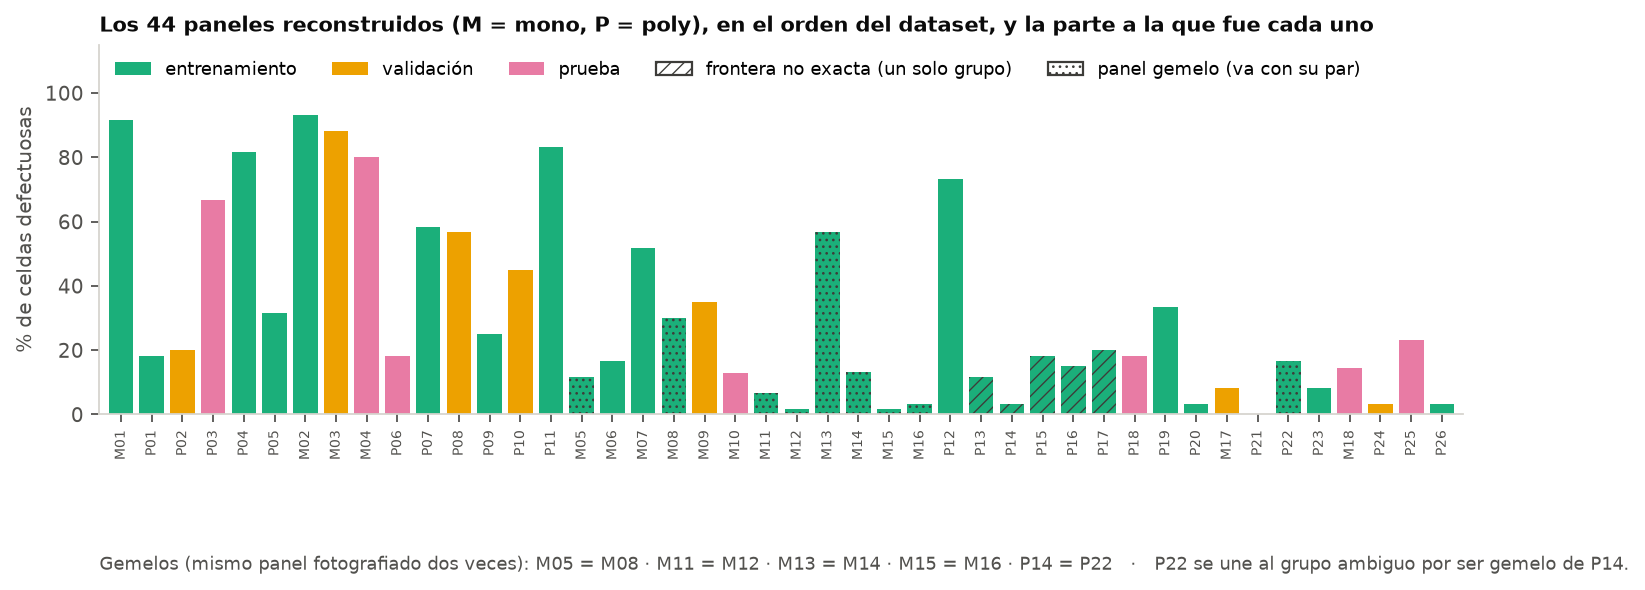
\includegraphics[width=0.8\textwidth]{p2_paneles_particion.png}

  \vspace{0.05cm}
  \footnotesize
  \begin{tabular}{@{}l rrrrr@{}}
    \toprule
    Parte & Paneles & Celdas & Mono & Poly & \% defectuosas \\
    \midrule
    Entrenamiento & 30 & 1.790 & 720 & 1.070 & 29,5 \\
    Validación & 7 & 432 & 192 & 240 & 35,9 \\
    Prueba & 7 & 402 & 162 & 240 & 34,3 \\
    \bottomrule
  \end{tabular}
\end{frame}

% ------------------------------------------------------------------ 4 fuga
\begin{frame}{La partición por panel no tiene fuga}{3 · Métodos y resultados · Control de fuga}
  \begin{columns}[c]
    \begin{column}{0.5\textwidth}
      \cab{Qué medimos}
      \small Celdas consecutivas de un panel salen de obleas vecinas y son casi idénticas. Si quedan en partes distintas, el modelo puede acertar
      \emph{reconociendo el panel}. Contamos los pares con correlación alta que quedan repartidos, frente a una partición al azar por celda.\par
      \vspace{0.3cm}
      También encontramos \textbf{5 pares de paneles gemelos}, el mismo panel fotografiado dos veces. Van siempre juntos.
    \end{column}
    \begin{column}{0.45\textwidth}
      \centering
      \begin{tabular}{@{}l rr@{}}
        \toprule
        Pares entre partes & Por panel & Al azar \\
        \midrule
        $r>0{,}95$ (1.193) & \textbf{\color{ud}\Large 0} & {\Large 498} \\[3pt]
        $r>0{,}90$ (4.118) & 7 & 1.769 \\
        \bottomrule
      \end{tabular}
      \vspace{0.3cm}

      {\small\color{gris}Es la prueba que fijó la propuesta (§5.1): la reconstrucción de paneles funcionó.}
    \end{column}
  \end{columns}
\end{frame}

% ------------------------------------------------------------------ 5 máscara
\begin{frame}{Máscara v1: recupera las celdas casi apagadas}{3 · Métodos y resultados · Máscara}
  \begin{columns}[c]
    \begin{column}{0.62\textwidth}
      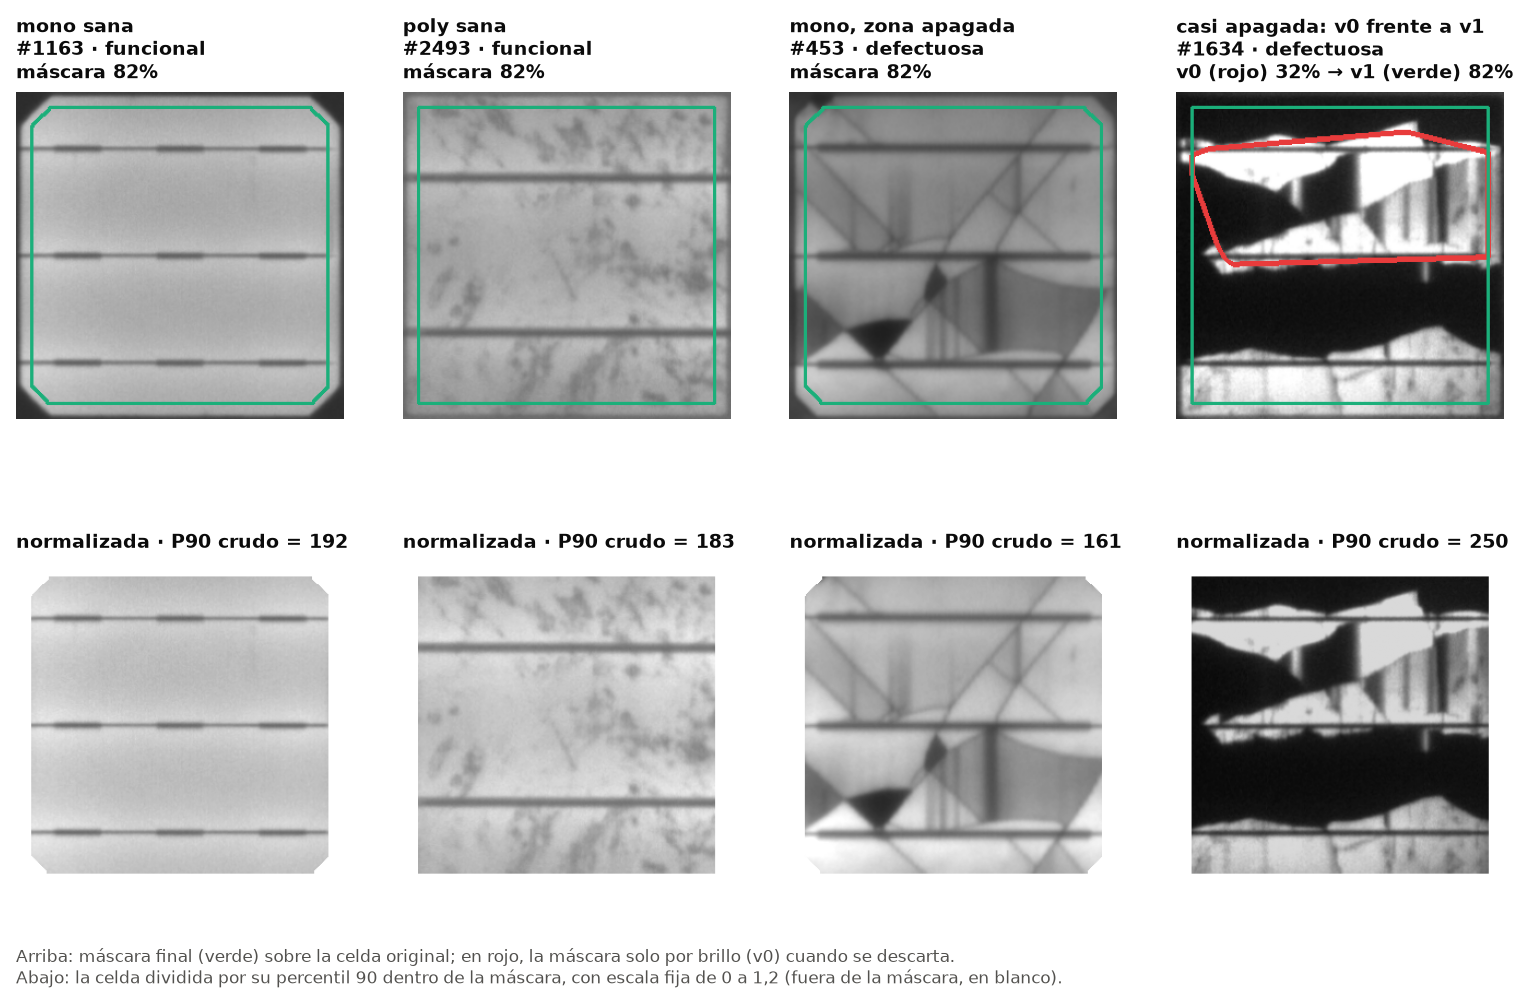
\includegraphics[width=\linewidth]{n2_mascara_ejemplos.png}
    \end{column}
    \begin{column}{0.36\textwidth}
      \footnotesize
      \cab{El problema}
      Si la zona apagada es muy grande, el umbral la saca de la máscara (rojo).\par\vspace{0.15cm}
      \cab{El cambio}
      Si la máscara cubre menos del 90\,\% de la plantilla del tipo, se usa la plantilla.\par\vspace{0.15cm}
      \cab{A quién afecta}
      \textbf{17 celdas}, todas poly, defectuosas y de entrenamiento. La mínima pasa de 32\,\% a 74\,\%.
    \end{column}
  \end{columns}
\end{frame}

% ------------------------------------------------------------------ 6 normalización
\begin{frame}{La normalización iguala los paneles}{3 · Métodos y resultados · Normalización}
  \centering
  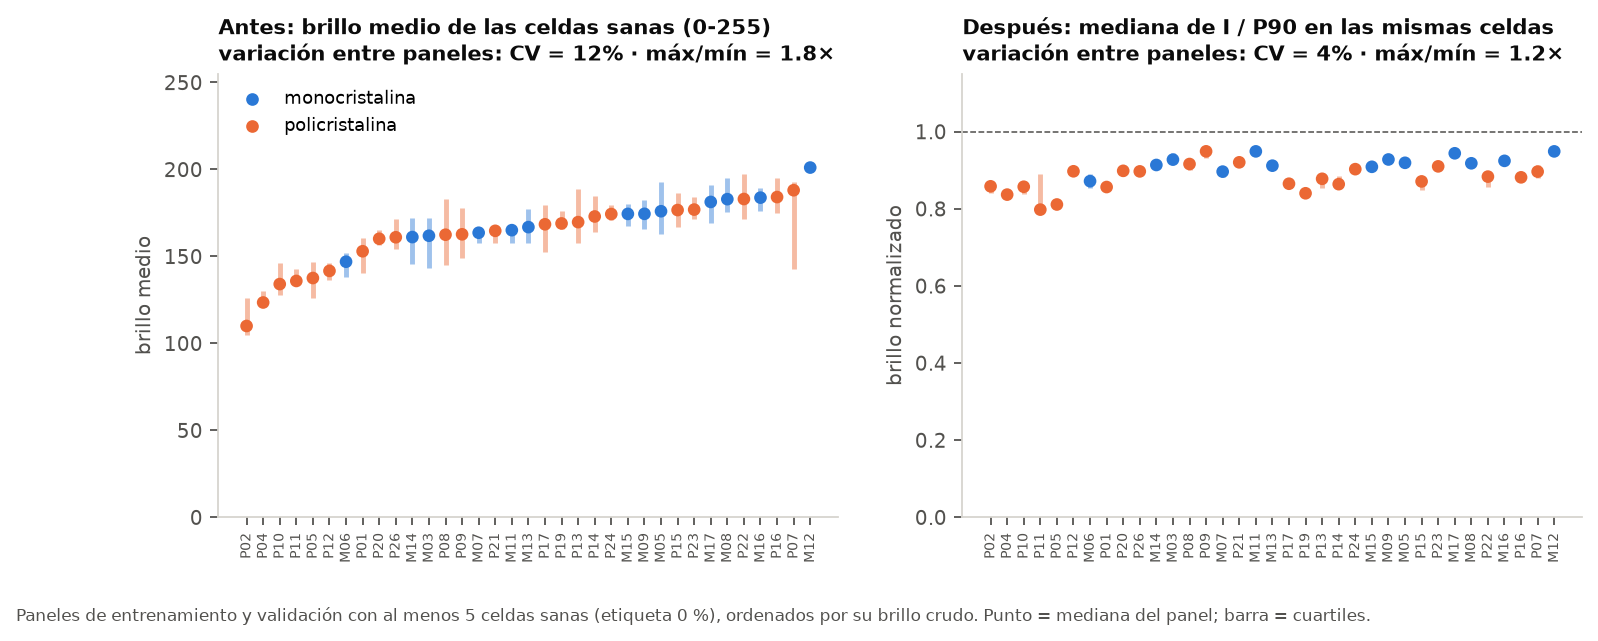
\includegraphics[width=0.86\textwidth]{n1_normalizacion_paneles.png}

  \vspace{0.05cm}
  \begin{columns}[c]
    \begin{column}{0.4\textwidth}
      \small
      \[ I_n(x,y)=\frac{I(x,y)}{P_{90}\{I(p):p\in M\}} \]
    \end{column}
    \begin{column}{0.56\textwidth}
      \footnotesize
      \begin{tabular}{@{}l ccc@{}}
        \toprule
        CV entre paneles & Todas & Mono & Poly \\
        \midrule
        Antes & 11,6\,\% & 7,6\,\% & 12,7\,\% \\
        Después & \textbf{\color{ud}4,1\,\%} & 2,2\,\% & 4,0\,\% \\
        \bottomrule
      \end{tabular}
    \end{column}
  \end{columns}
\end{frame}

% ------------------------------------------------------------------ 7 hallazgo
\begin{frame}{Hallazgo: el brillo crudo delata al panel}{3 · Métodos y resultados · Exposición}
  \centering
  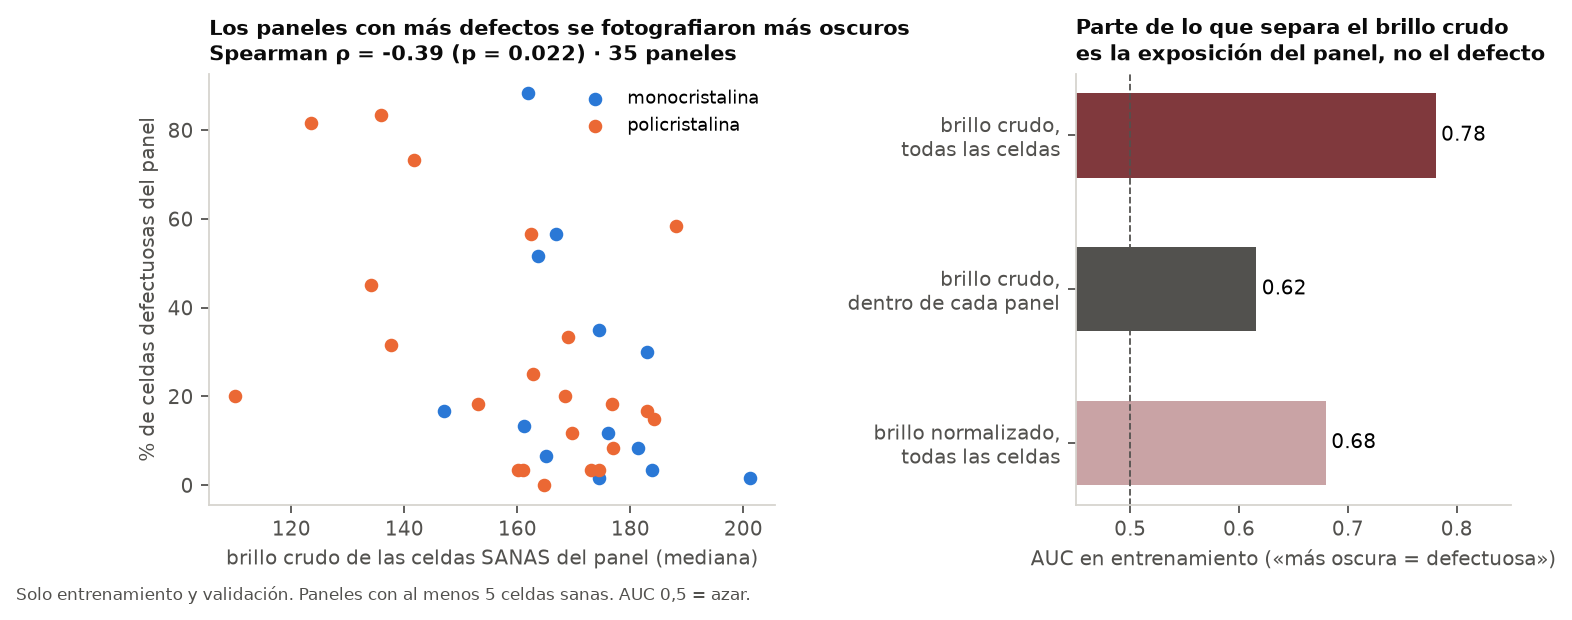
\includegraphics[width=0.8\textwidth]{n3_brillo_atajo_panel.png}

  \vspace{0.1cm}
  \raggedright\small
  Los paneles más dañados se fotografiaron más oscuros. Un modelo que use el brillo crudo aprende en parte \emph{«este panel es oscuro»}: eso no es un defecto,
  y con otra cámara no serviría. \textbf{Por eso la red solo verá imágenes normalizadas.}
\end{frame}

% ------------------------------------------------------------------ 8 línea base
\begin{frame}{Línea base en validación: mono va bien, poly no}{3 · Métodos y resultados · Línea base}
  \centering
  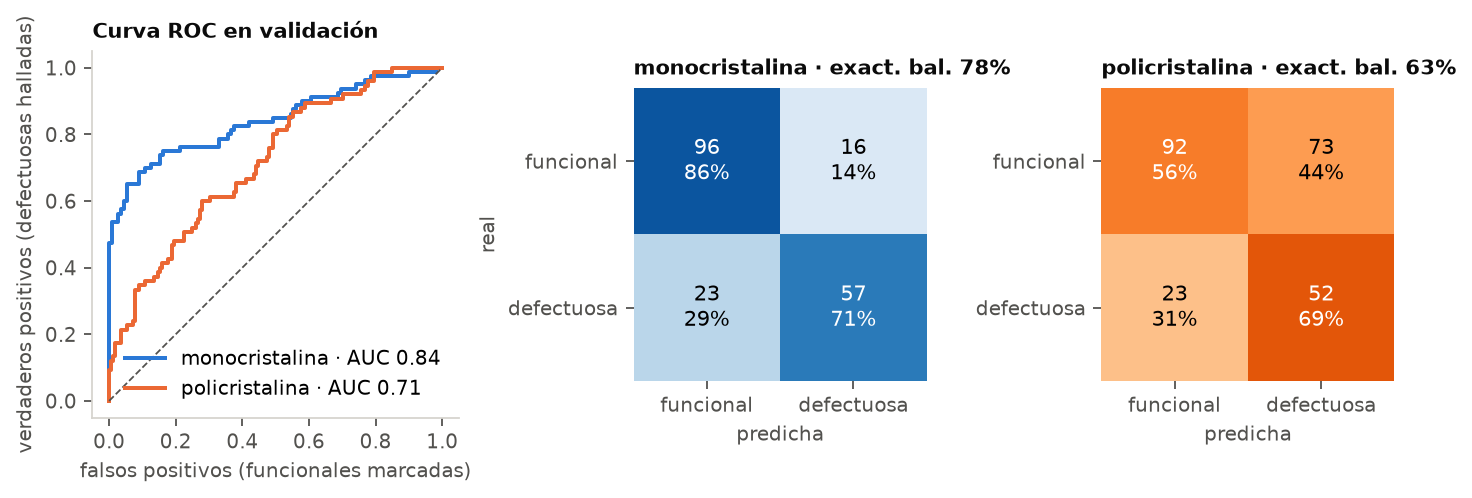
\includegraphics[width=0.72\textwidth]{f4_linea_base_val.png}

  \vspace{0.05cm}
  \footnotesize
  \begin{tabular}{@{}l ccc c ccc@{}}
    \toprule
    & \multicolumn{3}{c}{Con brillo crudo} & & \multicolumn{3}{c}{Sin brillo crudo} \\
    \cmidrule(lr){2-4}\cmidrule(lr){6-8}
    & AUC & Exact. bal. & F1 def. & & AUC & Exact. bal. & F1 def. \\
    \midrule
    Mono & 0,84 & 78,5\,\% & 0,75 & & 0,78 & 66,3\,\% & 0,64 \\
    Poly & 0,71 & 62,5\,\% & 0,52 & & 0,67 & 65,7\,\% & 0,53 \\
    Todas & \textbf{0,78} & 69,1\,\% & 0,62 & & 0,73 & 67,3\,\% & 0,59 \\
    \bottomrule
  \end{tabular}
\end{frame}

% ------------------------------------------------------------------ 9 dónde falla
\begin{frame}{Dónde falla la línea base, y qué semana lo ataca}{3 · Métodos y resultados · Errores}
  \begin{columns}[c]
    \begin{column}{0.6\textwidth}
      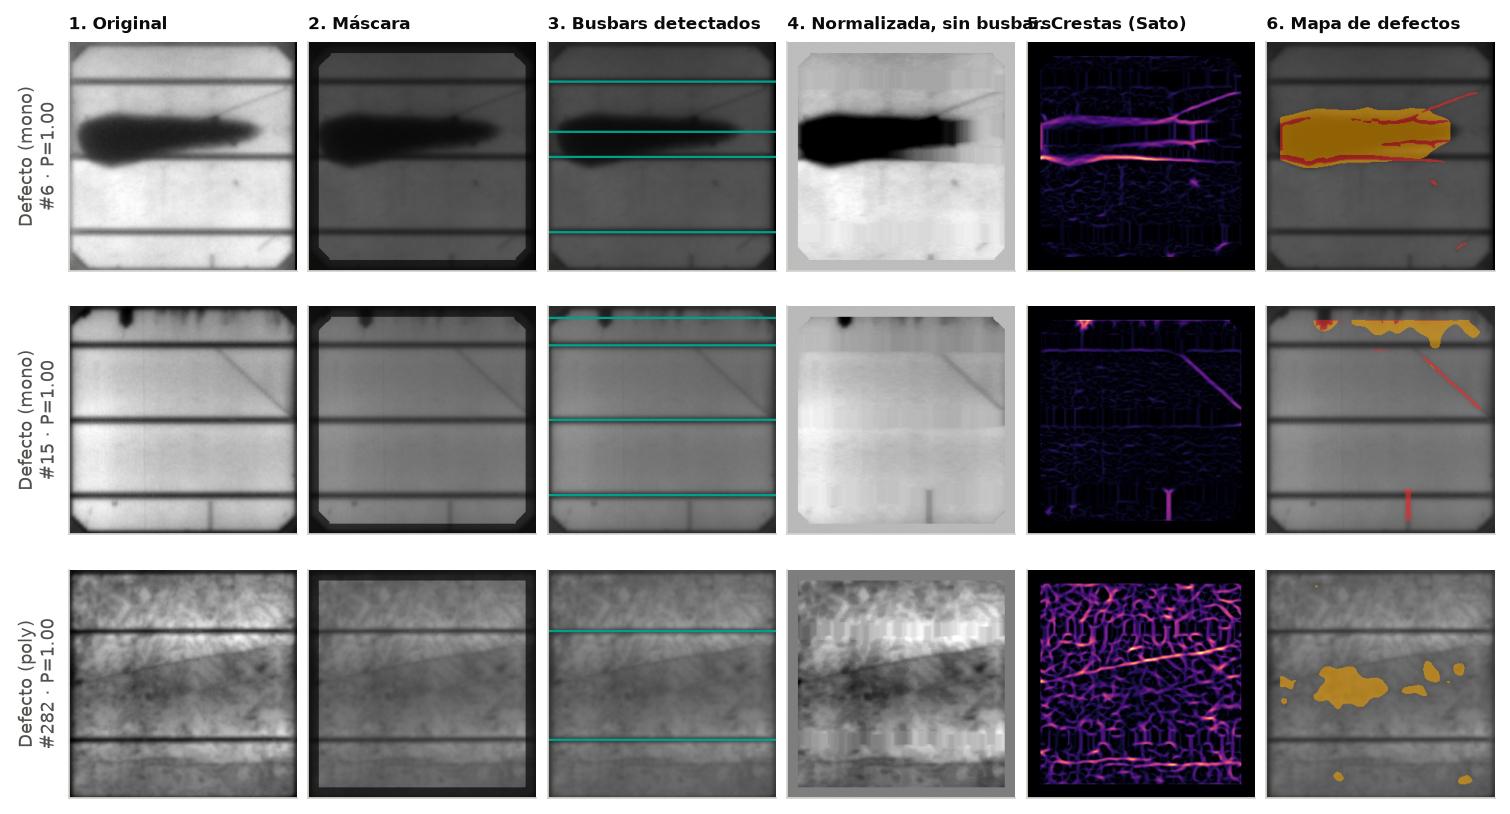
\includegraphics[width=\linewidth]{f2_pipeline_pasos.png}
    \end{column}
    \begin{column}{0.38\textwidth}
      \footnotesize
      \cab{Fila 1 · falso busbar}
      Una mancha grande se toma por busbar y el cierre la rellena a medias. \textbf{$\rightarrow$ Semana 2}\par\vspace{0.12cm}
      \cab{Fila 3 · granos de poly}
      Sato responde a los bordes de grano: en poly, 73 de 165 funcionales salen marcadas. \textbf{$\rightarrow$ Semana 3}\par\vspace{0.12cm}
      \cab{Contexto}
      Con partición al azar, esta línea base daba AUC 0,84. El artículo de referencia (88,42\,\% con CNN) también parte al azar [1].
    \end{column}
  \end{columns}
\end{frame}

% ------------------------------------------------------------------ 10 decisiones y riesgos
\begin{frame}{Decisiones y riesgos}{5 · Decisiones · 6 · Riesgos}
  \begin{columns}[t]
    \begin{column}{0.48\textwidth}
      \cab{Decidimos}
      \small
      \begin{itemize}
        \item Máscara v1 con respaldo de plantilla. Es un ajuste dentro de §4.1.
        \item Línea base reportada con y sin brillo crudo. La CNN no lo recibe.
        \item Métricas balanceadas y por tipo desde ya: validación tiene 36\,\% de defectuosas y entrenamiento 30\,\%.
      \end{itemize}
      \vspace{0.15cm}
      {\color{ud}\bfseries Sin cambios al alcance ni a los objetivos.} La prueba no se ha usado.
    \end{column}
    \begin{column}{0.48\textwidth}
      \cab{Vigilamos}
      \small
      \begin{itemize}
        \item \textbf{Granos de poly}: Gabor y filtrado por orientación y longitud (S3).
        \item \textbf{Falsos busbars}: banda fina y de todo el ancho (S2).
        \item \textbf{Celdas con 2 busbars}: verificar el notch en ellas (S2).
        \item \textbf{GPU de 4 GB}: alcanza para la CNN pequeña; Colab si hiciera falta.
      \end{itemize}
    \end{column}
  \end{columns}
\end{frame}

% ------------------------------------------------------------------ 11 plan
\begin{frame}{Semana 2: quitar los busbars de dos formas}{7 · Plan de la semana siguiente}
  \begin{columns}[t]
    \begin{column}{0.47\textwidth}
      \cab{A · Notch gaussiano (lab 9)}
      \small Agujeros gaussianos en $\pm k v_0$ sobre el eje vertical del espectro, sin tocar DC. Dos variantes: en toda la celda y solo en las filas de busbar.
      \[ I_A=\mathcal{F}^{-1}\{H(u,v)\,F(u,v)\} \]
    \end{column}
    \begin{column}{0.47\textwidth}
      \cab{B · Cierre morfológico (lab 10)}
      \small Elemento vertical más alto que la banda, solo en las filas detectadas, exigiendo que la banda sea fina y de todo el ancho.
      \[ I_B=I_n\bullet B=(I_n\oplus B)\ominus B \]
    \end{column}
  \end{columns}
  \vspace{0.15cm}
  \small
  \textbf{Se compara en validación} con los criterios de imagen de la tabla 3: brillo residual en las filas del busbar, cambio fuera de ellas y tiempo por celda.
  También se revisan las grietas verticales finas al quitar los dedos. \textbf{El criterio que decide}, el AUC de la CNN con cada alternativa, se mide en la semana 3.
\end{frame}

{\setbeamercolor{background canvas}{bg=ud}
\begin{frame}[plain]
  \begin{tikzpicture}[remember picture,overlay]
    \node[anchor=north west] at ([xshift=0.6cm,yshift=-0.35cm]current page.north west)
      {
\includegraphics[height=1.15cm]{logo_blanco.png}};
  \end{tikzpicture}
  \centering\color{white}
  \vspace{1.2cm}
  {\Huge Preguntas}\par\vspace{0.4cm}
  {\large\itshape Código y cifras: etiqueta \texttt{avance-1} del repositorio.}\par\vspace{0.8cm}
  {\footnotesize [1] S. Deitsch \emph{et al.}, «Automatic classification of defective photovoltaic module cells in electroluminescence images»,
  \emph{Solar Energy}, vol. 185, 2019. · Imágenes ELPV, CC BY-NC-SA 4.0.}
\end{frame}}

\end{document}
